% Created 2019-09-25 Wed 00:34
% Intended LaTeX compiler: pdflatex
\documentclass[10pt,t]{beamer}
\usepackage[utf8]{inputenc}
\usepackage[T1]{fontenc}
\usepackage{graphicx}
\usepackage{grffile}
\usepackage{longtable}
\usepackage{wrapfig}
\usepackage{rotating}
\usepackage{amsmath}
\usepackage{textcomp}
\usepackage{amssymb}
\usepackage{capt-of}
\usepackage{hyperref}
\usetheme{default}
\author{L. Larrabee Strow and Howard Motteler (UMBC)}
\date{\today}
\title{\large Validation of the AIRS L1c Radiance Product: Spectral and Radiometric}
\subtitle{\footnotesize{AIRS Science Team Meeting}}
\date{\vspace{0.1in}\footnotesize{September 25, 2019\vfill}}
\author{L. Larrabee Strow\inst{1,2} and Howard Motteler\inst{2}}
\institute[UMBC]{\inst{1} UMBC Physics Dept. \and \inst{2}UMBC JCET}
\input beamer_setup
\usetheme{metropolis}
\metroset{titleformat title=allcaps}
\renewcommand{\UrlFont}{\small\tt}
\renewcommand*{\UrlFont}{\footnotesize}
\tolerance=1000
\RequirePackage{fancyvrb}
\DefineVerbatimEnvironment{verbatim}{Verbatim}{fontsize=\footnotesize}
\author{L.~Larrabee~Strow and Howard Motteler (UMBC)}
\hypersetup{
 pdfauthor={L. Larrabee Strow and Howard Motteler (UMBC)},
 pdftitle={\large Validation of the AIRS L1c Radiance Product: Spectral and Radiometric},
 pdfkeywords={},
 pdfsubject={},
 pdfcreator={Emacs 26.1 (Org mode 9.2)}, 
 pdflang={English}}
\begin{document}

\maketitle
\addtobeamertemplate{block begin}{
  \setlength{\parsep}{0pt}
  \setlength{\topsep}{3pt plus 2pt minus 2.5pt}
  \setlength{\itemsep}{0pt plus 0pt minus 2pt}
  \setlength{\partopsep}{2pt}
}

\begin{frame}[label={sec:orgb6b6e7f}]{Overview}
\begin{itemize}
\item Radiometric validation of L1c "fill" channels
\item Radiometric corrections for:
\begin{itemize}
\item Instrument frequency drifts
\item Doppler effect
\end{itemize}
\end{itemize}

In general, L1c radiances are identical to L1b radiance, except for frequency shift corrections, unless there are significant errors due to:
\begin{itemize}
\item Detector popping
\item C\textsubscript{ij} errors (inhomogenous scenes)
\item Poor detector performance (high noise, continuous popping, etc.)
\end{itemize}

L1c contains "fill channels" that do not exist in L1b to cover frequency gaps.   This algorithm was developed by George Aumann and Evan Manning using simulated spectra provided by Sergio DeSouza-Machado.
\end{frame}

\begin{frame}[label={sec:orga5ec514}]{L1c Characteristics}
\begin{itemize}
\item Creates visually appealing spectra
\item However, in general channels that are routinely corrected, and fill channels should not be used for science applications
\item Fill channels are used to create the CHIRP ILS radiance product, but only for a few channels that are weakly dependent on the fill channel radiance
\item The CHIRP application does require us to have a nominal value for the accuracy of the fill channel radiances
\end{itemize}
\end{frame}

\begin{frame}[label={sec:org3ce0780},shrink=10]{Grating Equation: Model Used for Frequeny Shifting}
Basic equation for channel frequency:

\begin{displaymath}
\nu_i = \frac{m}{d(\sin(\alpha_i) + \sin(\beta_i))}
\end{displaymath}
where 
\(\alpha\)\textsubscript{i} = incidence angle, \(\beta\)\textsubscript{i} = diffracted angle, d = groove spacing, and m = grating order. 

The angle of diffraction is computed from the linear positions \(y\) of the detectors on the focal using,

\begin{displaymath}
\beta_i = \tan^{-1}(y/F)
\end{displaymath}

where \(y = y_o + i*ds\). F = focal length of condensing mirror, \(ds\) is the detector spacing on the detector array, and \(i\) is the index nunber of the detector.  We often call \(y\) "yoffset".

We measure \(y_o\) for each array, which varies with orbit phase and time.  The time dependence includes secular, exponential, and. seasonal terms.  The season terms are related to the satellite solar \(\beta\) angle.
\end{frame}

\begin{frame}[label={sec:org8a960e1}]{Deriving AIRS Frequency Shifts}
\begin{itemize}
\item Both the Doppler shifts and the instrument frequency shifts are measured by cross-correlating the observed spectral with spectral computed from the ERA reanalysisl
\item We shift the computed spectra over a range of values.  The AIRS true frequency scale is the same as the ERA computed scale when the cross-correlation reaches a maximum
\item For the time dependence of the instrument frequency drifts we generally use an array in the water band that retains high spectral contrast over most observing conditions.
\end{itemize}
\end{frame}
\begin{frame}[label={sec:org20efd55}]{B(T) Sensitivity to Yoffsets}
Max B(T) changes over (a) Mission, (b) Daily (orbit phase)

\begin{center}
\includegraphics[width=0.8\linewidth]{./Figsc/Pdf/max_mission_max_daily_diff_in_bt.pdf}
\end{center}
\end{frame}

\begin{frame}[label={sec:org7417adb}]{Yoffset is Retrieved from Observations}
\begin{itemize}
\item yoffset as a function of time and orbit phase
\end{itemize}

\begin{center}
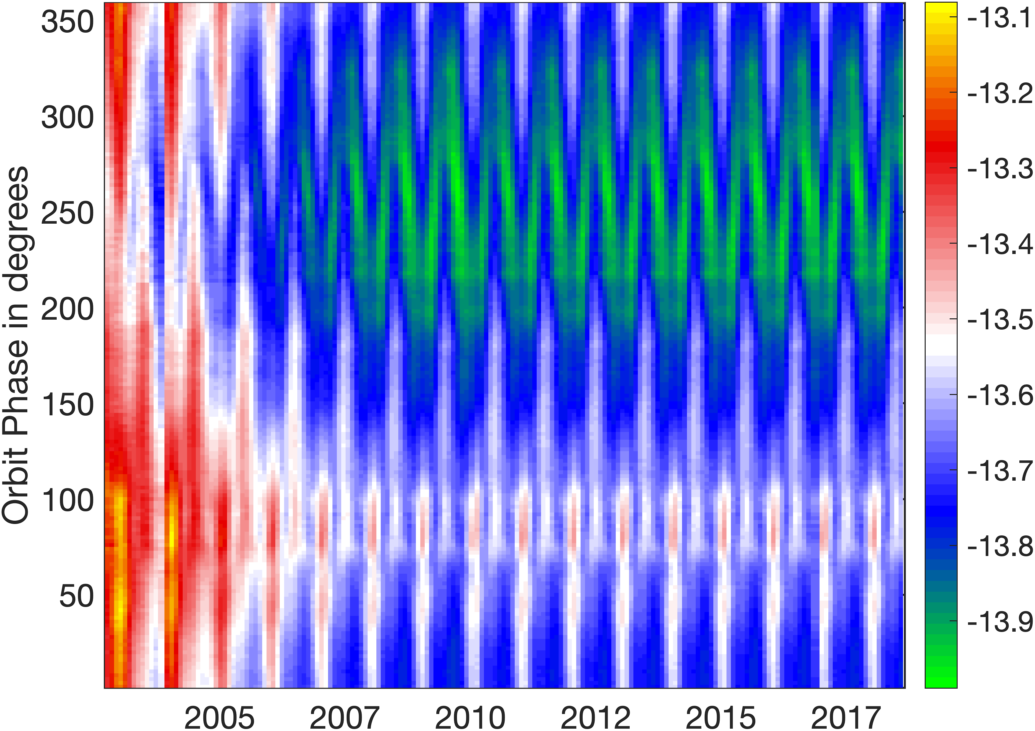
\includegraphics[width=0.8\linewidth]{./Figs/Png/offset_time_phase_pcolor.png}
\end{center}
\end{frame}

\begin{frame}[label={sec:org0a50681}]{L1c Yoffsets}
\begin{itemize}
\item Descending equator
\item Raw L1c (no \(\nu\) calibration)
\item L1c adjusted to new fixed L1c \(\nu\) grid
\end{itemize}

\begin{center}
\includegraphics[width=0.7\linewidth]{./Figsc/Pdf/l1c_nu_cal_closure_m3.pdf}
\end{center}
\end{frame}

\begin{frame}[label={sec:orgdef5d0f}]{M3 Results: Descending, All Latitudes}
\begin{center}
\includegraphics[width=0.7\linewidth]{./Figsc/Pdf/all_m3_desc_obs_cal.pdf}
\end{center}
\end{frame}

\begin{frame}[label={sec:orgee3f6a8}]{M10 Results}
\begin{center}
\includegraphics[width=0.7\linewidth]{./Figsc/Pdf/m10_desc_and_asc_cal_obs_lat7_m1p4deg.pdf}
\end{center}
\end{frame}

\begin{frame}[label={sec:orgbad9e2c}]{M4a Results}
\begin{center}
\includegraphics[width=0.7\linewidth]{./Figsc/Pdf/m4a_desc_and_asc_cal_obs_lat7_m1p4deg.pdf}
\end{center}
\end{frame}

\begin{frame}[label={sec:org9fed8c6},shrink=0]{Doppler Effect}
Fractional doppler shift given by:\\

\begin{displaymath}
\frac{\Omega R_e}{c} \sin(\theta_{zenith}) \cos(lat_{sub}) |sin(\theta_{azimuth})|
\end{displaymath}

\small where, \(\Omega\) = 7.292 \texttimes{} 10\textsuperscript{-5} (earth's rotational velocity, rad/sec) \\
R\_e = 6.3781 \texttimes{} 10\textsuperscript{8} (earth radius, cm) \\
c = 2.99792 \texttimes{} 10\textsuperscript{10}  (speed of light, cm/sec)\\

\vspace{0.2in}

\small See Yong Chen et.al.,  Applied Optics, September 2013
\end{frame}

\begin{frame}[label={sec:orgdcf87d6}]{Measurement of AIRS Doppler Shifts versus Latitude (M3)}
\begin{itemize}
\item Performed using cross-correlation with simulated radiances
\item Showing mean shift (xtrack(1:45) - xtrack(46:90))
\end{itemize}

\begin{center}
\includegraphics[width=0.7\linewidth]{./Figsc/Pdf/obs_vs_cal_ppm_diff_vs_lat_asc_desc_mean46to89_vs_mean2to45.pdf}
\end{center}
\end{frame}

\begin{frame}[label={sec:orgf37a025}]{Doppler Shifts versus Cross-Track Index (M3)}
\begin{columns}
\begin{column}{0.55\columnwidth}
\begin{block}{-1.4\textdegree{} Latitude}
\begin{center}
\includegraphics[width=\linewidth]{./Figsc/Pdf/obs_vs_cal_ppm_m1p4deg_lat_vs_xtrack.pdf}
\end{center}
\end{block}
\end{column}

\begin{column}{0.55\columnwidth}
\begin{block}{-39\textdegree{} Latitude}
\begin{center}
\includegraphics[width=\linewidth]{./Figsc/Pdf/obs_vs_cal_ppm_m39deg_lat_vs_xtrack.pdf}
\end{center}
\end{block}
\end{column}
\end{columns}
\end{frame}

\begin{frame}[label={sec:org8d76eaa}]{Doppler Shifts using M10 versus M3}
\vspace{-0.1in}
\begin{itemize}
\item How similar are Doppler shifts using M10 instead of M3?
\end{itemize}

\begin{center}
\includegraphics[width=0.7\linewidth]{./Figsc/Pdf/obs_vs_cal_ppm_m1p4deg_lat_vs_xtrack_with_m10_obs.pdf}
\end{center}
\vspace{-0.1in}
\begin{itemize}
\item \small M10 shifts have some curvature, but show same nominal behavior
\item \small Other studies indicate M3 is best for high-quality frequency shifts
\end{itemize}
\end{frame}

\begin{frame}[label={sec:orgac88f2b}]{Doppler Shift Closure Exercise}
\vspace{-0.1in}
\begin{itemize}
\item Apply theoretical Doppler shifts to data and re-measure observed shifts
\end{itemize}

\begin{center}
\includegraphics[width=0.7\linewidth]{./Figsc/Pdf/obs_vs_cal_ppm_m1p4deg_lat_vs_xtrack_with_closure.pdf}
\end{center}
\vspace{-0.1in}
\begin{itemize}
\item \small Reasonably good closure achieved
\end{itemize}
\end{frame}

\begin{frame}[label={sec:org5c19f92}]{Subtract Ascending from Descending for Full Range}
\vspace{-0.1in}
\begin{center}
\includegraphics[width=0.8\linewidth]{./Figsc/Pdf/sec_asym_bias_and_corr_desc_minus_asc_dc_removed_m45top41_lat.pdf}
\end{center}

\vspace{-0.15in}

\begin{itemize}
\item \small This is \textpm{}45\textdegree{} latitude average
\item \small Hash phases different for corrected L1c than un-corrected (see zooms)
\end{itemize}
\end{frame}

\begin{frame}[label={sec:org9359b0c}]{Validation of L1c Fill Channels}
\begin{itemize}
\item Use IASI and AIRS SNOs
\item Convert IASI to the AIRS ILS
\item Compare IASI2AIRS radiances to AIRS L1c
\end{itemize}
\end{frame}
\begin{frame}[label={sec:org2ec2273}]{Native Resolution Spectra}
\begin{center}
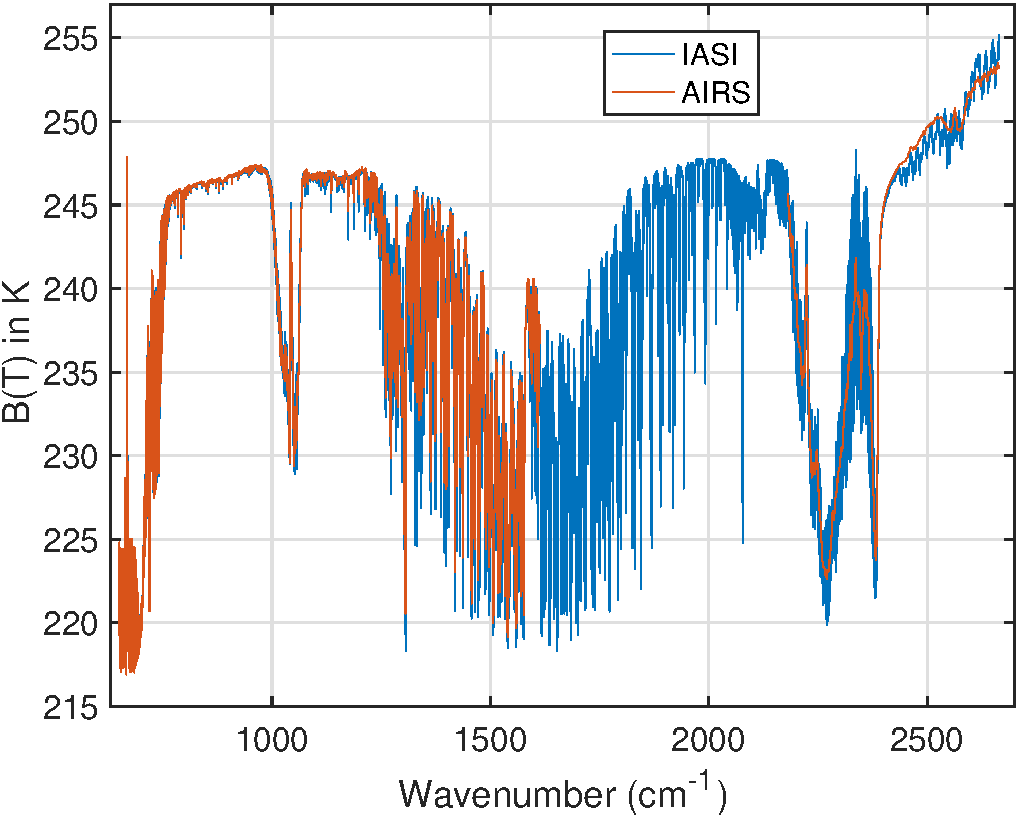
\includegraphics[width=0.8\linewidth]{./Figs/Pdf/airs_iasi_sno_native.pdf}
\end{center}
\end{frame}
\begin{frame}[label={sec:org7b222d0}]{Native Resolution Spectra with Fill Channels Marked}
\begin{center}
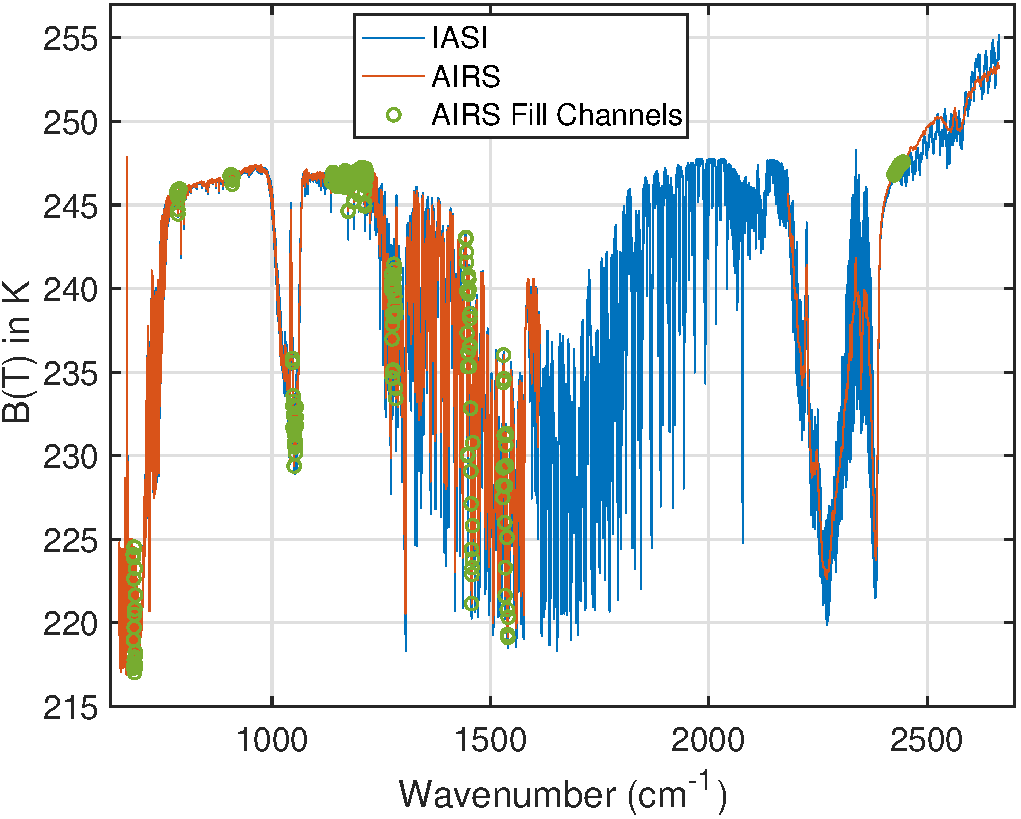
\includegraphics[width=0.8\linewidth]{./Figs/Pdf/airs_iasi_sno_native_with_fill_marked.pdf}
\end{center}
\end{frame}
\begin{frame}[label={sec:orge73e5cb}]{Zoom in Midwave}
\begin{center}
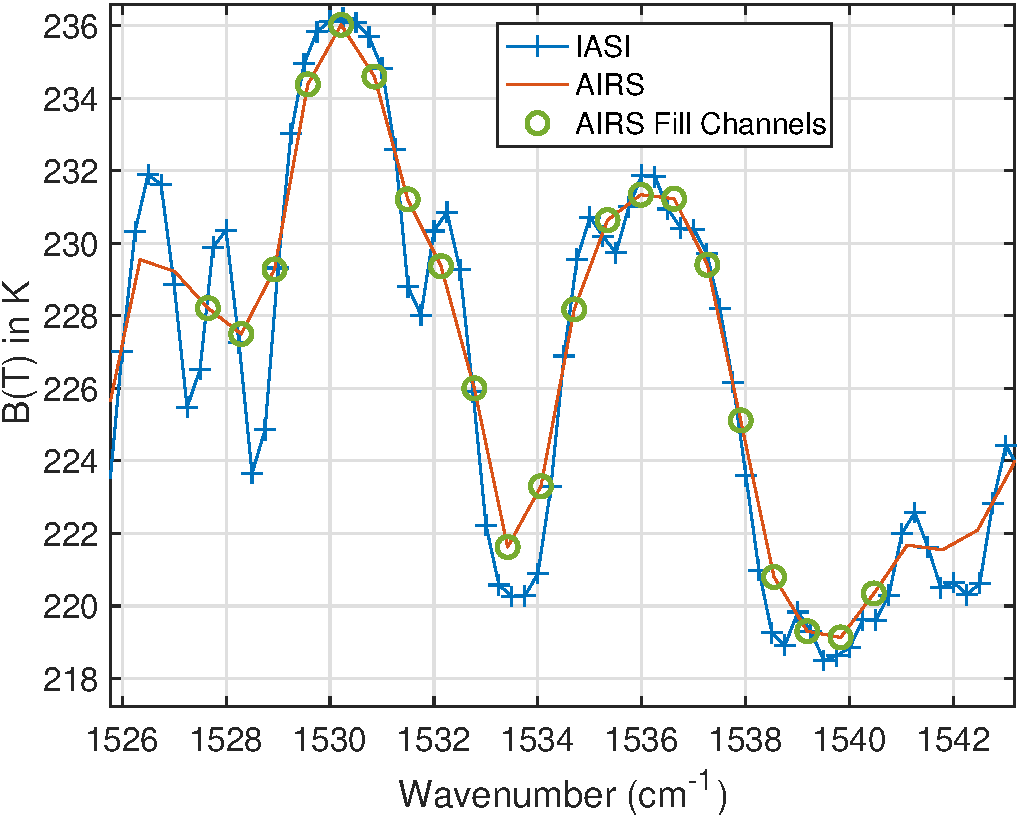
\includegraphics[width=0.8\linewidth]{./Figs/Pdf/airs_iasi_sno_native_with_fill_marked_mwzoom5.pdf}
\end{center}
\end{frame}
\begin{frame}[label={sec:orgd2f9278}]{Now Convert IASI to AIRS ILS and Compare}
\begin{center}
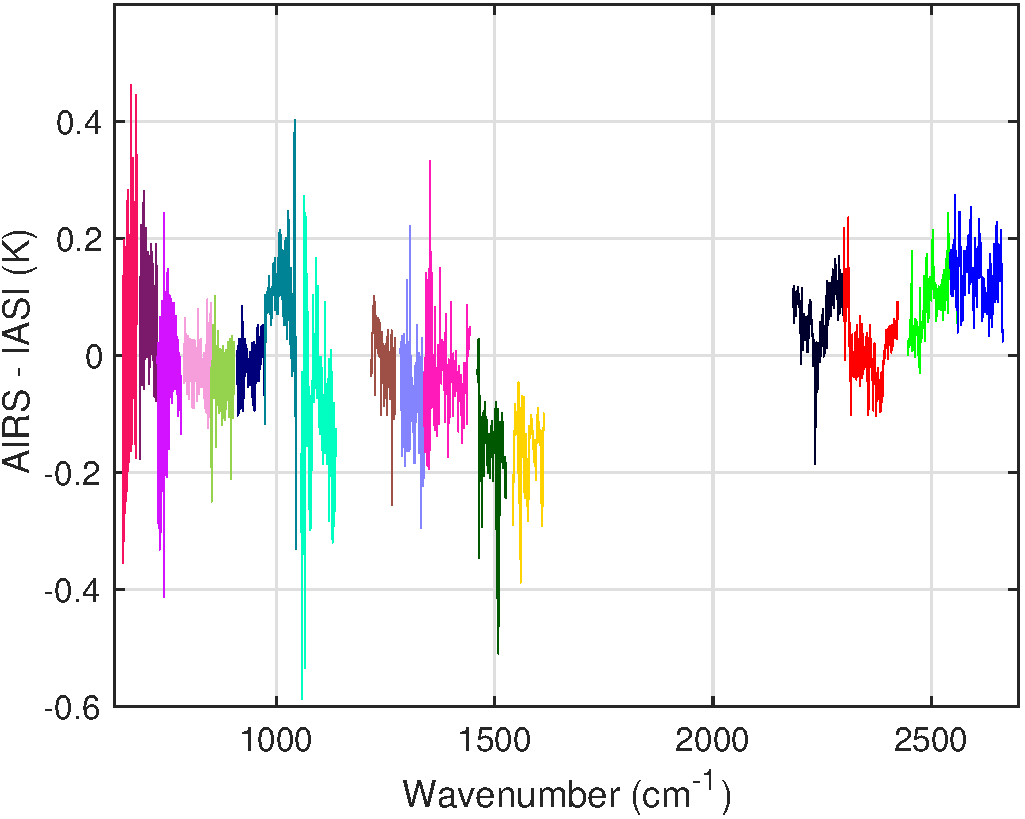
\includegraphics[width=0.8\linewidth]{./Figs/Pdf/sno_airs_m_iasi_no_fill.pdf}
\end{center}
\end{frame}
\begin{frame}[label={sec:org6c3a7f3}]{\small Now Convert IASI to AIRS ILS and Compare with Fill Channels}
\begin{center}
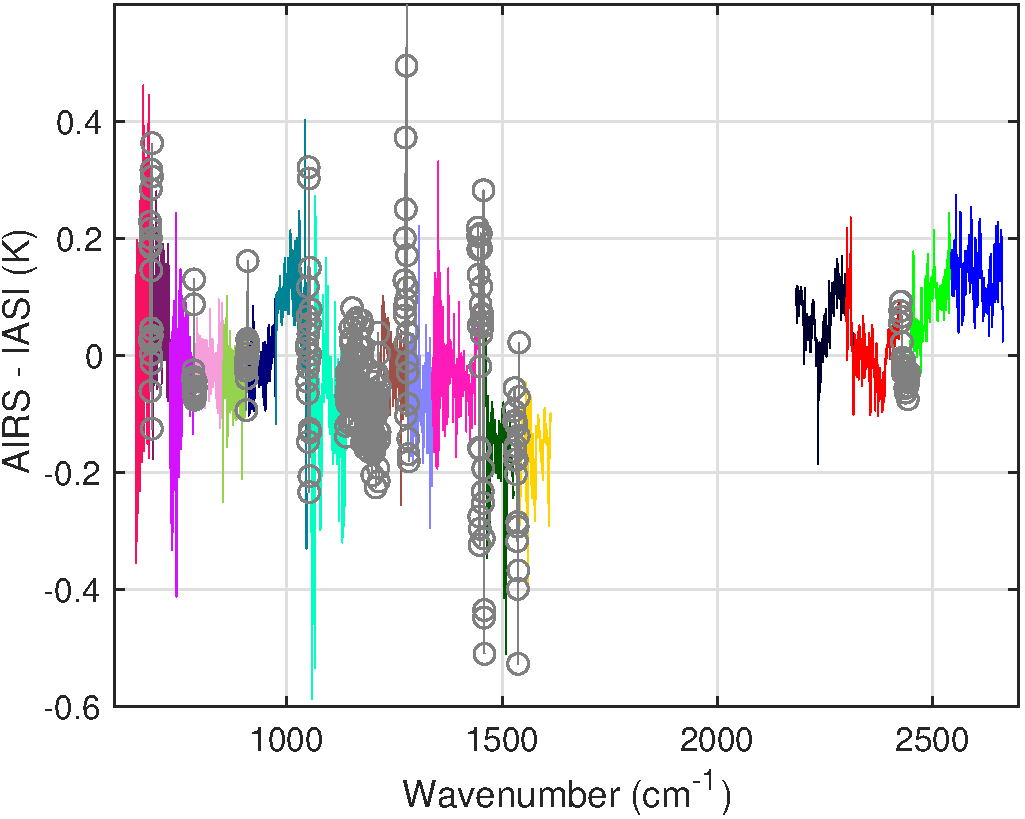
\includegraphics[width=0.8\linewidth]{./Figs/Pdf/sno_airs_m_iasi_with_fill.pdf}
\end{center}
\end{frame}
\begin{frame}[label={sec:org4f75b9a}]{Zooms of AIRS - IASI}
\begin{center}
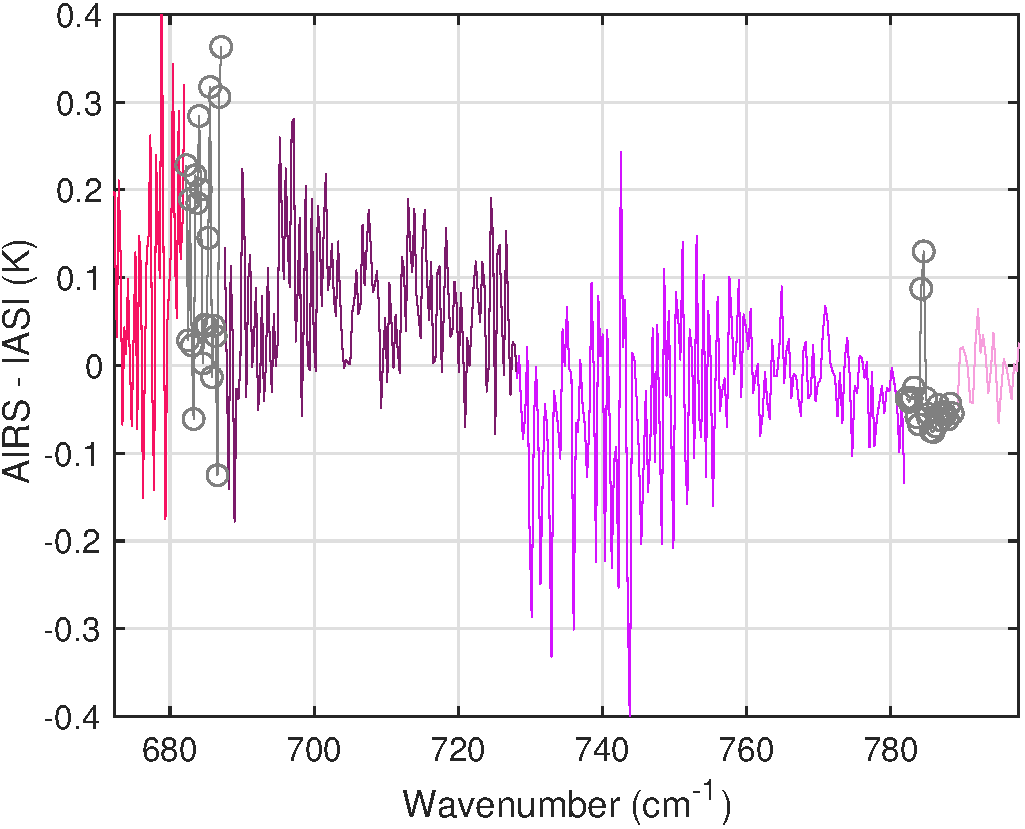
\includegraphics[width=.9\linewidth]{./Figs/Pdf/sno_airs_m_iasi_with_fill_lwzoom.pdf}
\end{center}
\end{frame}
\begin{frame}[label={sec:orgf5fd184}]{Zooms of AIRS - IASI}
\begin{center}
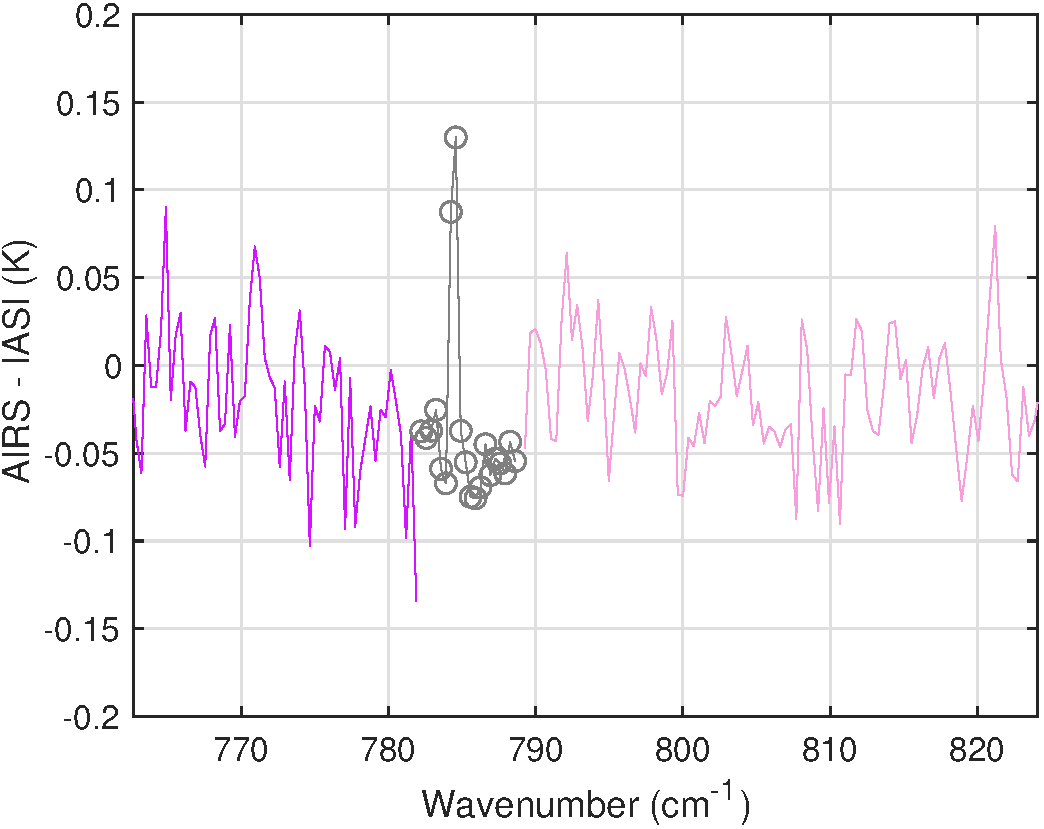
\includegraphics[width=0.8\linewidth]{./Figs/Pdf/sno_airs_m_iasi_with_fill_lwzoom2.pdf}
\end{center}
\end{frame}
\begin{frame}[label={sec:orgc41a381}]{Zooms of AIRS - IASI}
\begin{center}
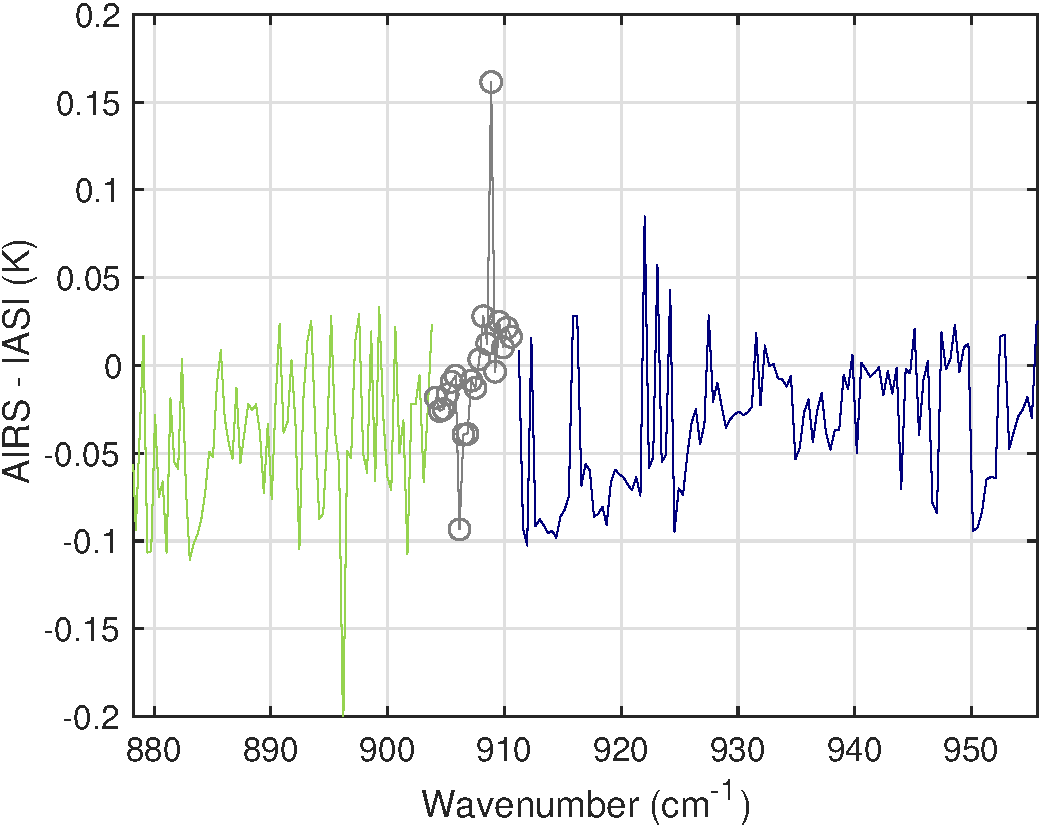
\includegraphics[width=0.8\linewidth]{./Figs/Pdf/sno_airs_m_iasi_with_fill_lwzoom3.pdf}
\end{center}
\end{frame}
\begin{frame}[label={sec:org53f6c55}]{Zooms of AIRS - IASI}
\begin{center}
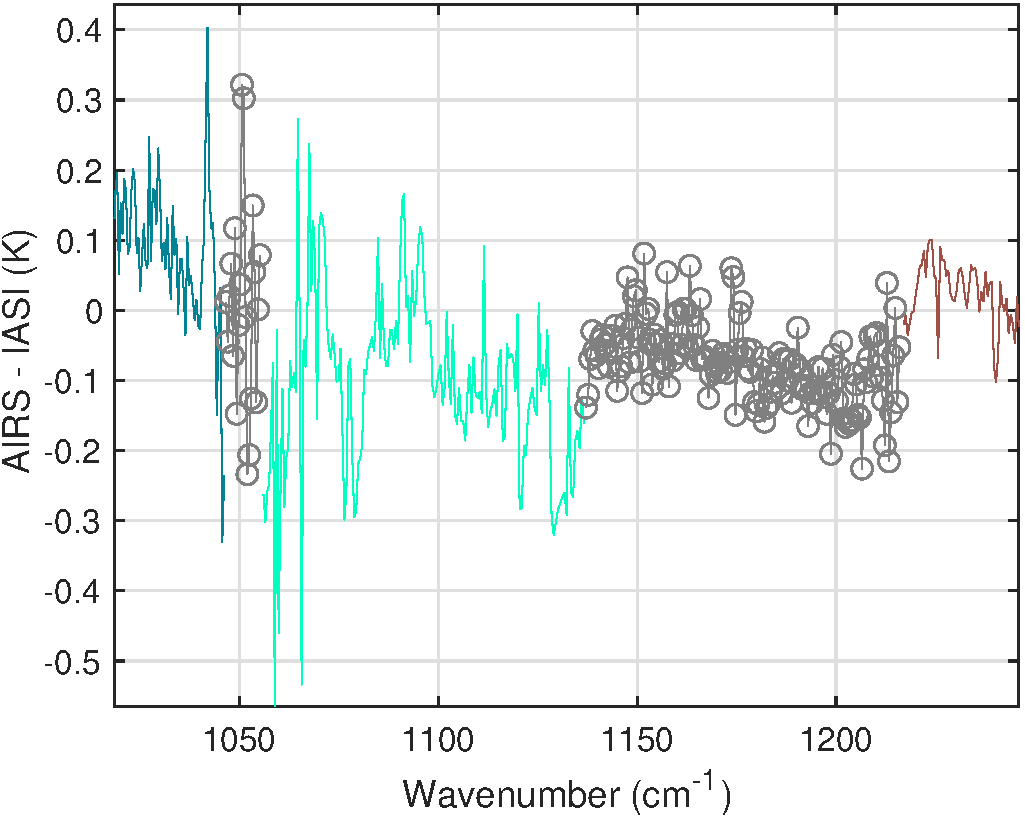
\includegraphics[width=0.8\linewidth]{./Figs/Pdf/sno_airs_m_iasi_with_fill_lwzoom4.pdf}
\end{center}
\end{frame}
\begin{frame}[label={sec:org1c87cfb}]{Zooms of AIRS - IASI}
\begin{center}
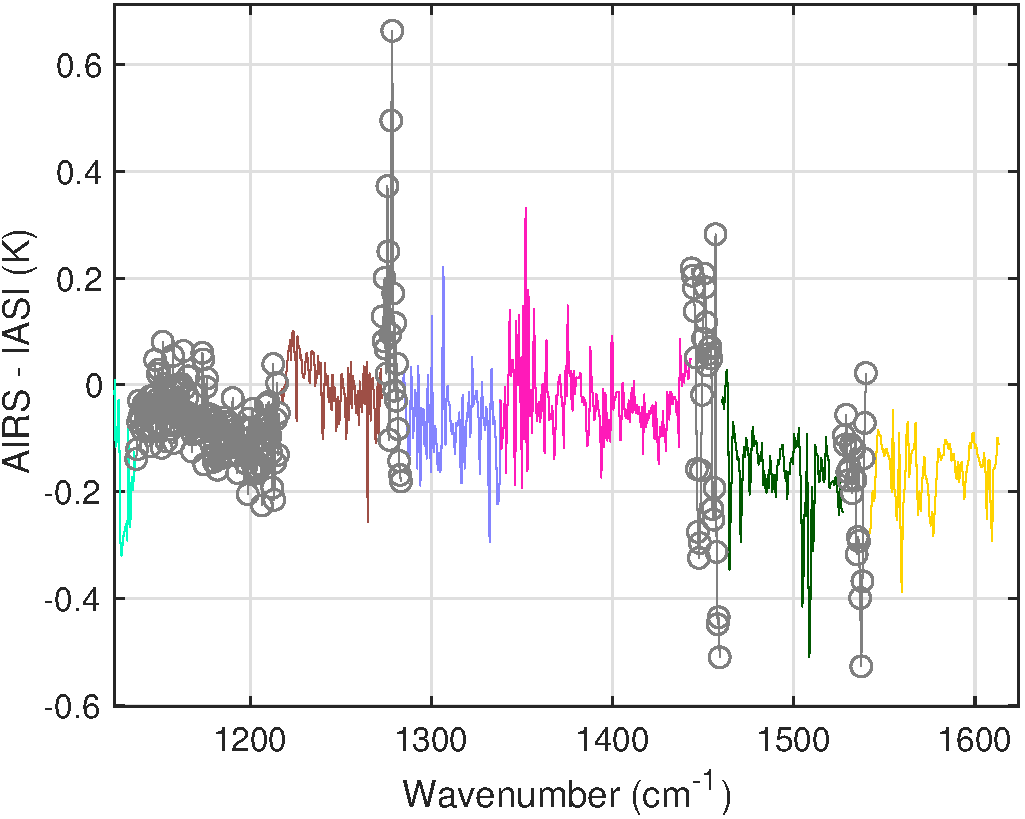
\includegraphics[width=0.8\linewidth]{./Figs/Pdf/sno_airs_m_iasi_with_fill_mwzoom5.pdf}
\end{center}
\end{frame}

\begin{frame}[label={sec:orgb3e8519}]{Conclusions}
\begin{itemize}
\item AIRS instrument frequency drifts largely eliminated in L1c
\item Some short-term problems in a few arrays after March 2014
\item Doppler effects largely removed
\item L1c fill channels radiances quite good!, sufficient for CHIRP
\item Except in mid-wave water, where some improvements might be nice
\end{itemize}

\begin{block}{User Visible Changes}
\begin{itemize}
\item New AIRS frequency scale!
\item 2650 channels
\item Retrievals need a new RTA 
\begin{itemize}
\item New L1c RTA exists
\item See talk by Chris Hepplewhite
\end{itemize}
\end{itemize}
\end{block}
\end{frame}
\end{document}